\section{Theorie}
\label{sec:Theorie}
Das Ziel dieses Versuches ist die präzise Messung der Hyperfeinstruktur- sowie
der Zeemann-Aufspaltung mit Hilfe der Methode des optischen Pumpens. Weiterhin sollen die Land\'{e}-
Faktoren von zwei Rubidium-Isotopen ermittelt werden.

In der Elektronenhülle eines Atoms können die Elektronen verschiedene Energieniveaus einnehmen.
Dabei wird immer der energetisch günstigste Zustand angestrebt, sodass die innersten Schalen
vollständig besetzt sind. Interessant für diesen Versuch sind die äußeren Niveaus, deren
Besetzung eine Temperaturabhängigkeit aufweist. Seien nun die beiden Energieniveaus
$W_{\mathrm{i}}$ und $W_{\mathrm{i}+1}$ ($W_{\mathrm{i}+1} >  W_{\mathrm{i}}$) gegeben.
Dann erfüllen diese die Boltzmannsche Gleichung
\begin{equation}
	\frac{N_{\mathrm{i}+1}}{N_{\mathrm{i}}} = \frac{g_{\mathrm{i}+1}}{g_{\mathrm{i}}} \frac{\exp(-W_{\mathrm{i}+1} / \mathrm{k}_{\mathrm{B}}T)}{\exp(-W_{\mathrm{i}} / \mathrm{k}_{\mathrm{B}}T)} \, \mathrm{,}
\end{equation}
wobei $g_{\mathrm{i}}$ dem statistischen Gewicht und $N_{\mathrm{i}}$ der Besetzungszahl
des jeweiligen Energieniveaus,
$\mathrm{k}_{\mathrm{B}}$ der Boltzmann-Konstanten \cite{k_b} und $T$ der Temperatur im thermischen
Gleichgewicht entspricht.
Im Normalfall sollte folglich $W_{\mathrm{i}}$ eine höhere Besetzungszahl aufweisen.
Mit dem optischen Pumpen wird eine Inversion ($N_{\mathrm{i}+1} > N_{\mathrm{i}}$) möglich.
Wenn diese Konstellation hergestellt wird, können Übergänge zwischen den beiden Niveaus
induziert werden, bei denen ein Photon mit der Energie
\begin{equation}
	h \nu = W_{\mathrm{i}+1} - W_{\mathrm{i}} \, \mathrm{,}
\end{equation}
emittiert wird. Die Frequenz wird hier $\nu$ genannt und $h$ entspricht dem Planckschen
Wirkungsquantum \cite{h}.

\subsection{Zusammenhang zwischen Drehimpuls, magnetischem Moment und Kernspin}

Die Elektronenhülle des Atoms besitzt einen Drehimpuls $\vec{J}$, der sich aus dem
Bahndrehimpuls $\vec{L}$ und dem Spin $\vec{S}$ zusammensetzt. An diesen koppelt das
zugehörige magnetische Moment
\begin{equation}
	\vec{\mu}_{\mathrm{J}} = - g_{\mathrm{J}} \mu_{\mathrm{B}} \vec{J} \, \mathrm{,}
\end{equation}
mit dem Bohrschen Magneton $\mu_{\mathrm{B}}$ \cite{mu_0} und dem Land\'{e}-Faktor $g_{\mathrm{J}}$.
Die Zusammensetzung des magnetischen Momentes der Elektronenhülle gemäß der
Russel-Saunders-Kopplung $\vec{\mu}_{\mathrm{J}} = \vec{\mu}_{\mathrm{L}} + \vec{\mu}_{\mathrm{S}}$ ermöglicht unter
Verwendung des Kosinussatzes den Ausdruck
\begin{equation}
	g_{\mathrm{J}} = \frac{3,0023 J(J+1) + 1,0023 (S(S+1)-L(L+1))}{2J(J+1)}
\end{equation}
für den Land\'{e}-Faktor.

Befindet sich das Atom in einem externen B-Feld, so tritt eine Aufspaltung der bisherigen
Energieniveaus ein. Dieser Effekt wird Zeemann-Effekt genannt.
Das B-Feld wirkt auf das magnetische Moment der Elektronenhülle und dieses führt eine Präzessionsbewegung
in Feldrichtung aus, wodurch sich eine Richtungsquantelung des Drehimpulses ergibt. Damit
ergibt sich die Wechselwirkungsenergie
\begin{equation}
	U_{\mathrm{mag}} = - \vec{\mu}_{\mathrm{J}} \cdot \vec{B} = M_{\mathrm{J}} g_{\mathrm{J}} \mu_{\mathrm{B}} B \, \mathrm{,} \, M_{\mathrm{J}} \in \{J \in \mathbb{Z} \, \vert -J \le M_{\mathrm{J}} \le J\} \, \mathrm{.}
\end{equation}
Die Orientierungsquantenzahl $M_{\mathrm{J}}$ folgt aus der Richtungsquantelung.

Bei dieser Überlegung wurde allerdings noch nicht der Einfluss des Kernspins berücksichtigt.
Der Gesamtdrehimpuls des Atoms ergibt sich nämlich durch eine Drehimpulsaddition von dem
Gesamtdrehimpuls der Elektronenhülle und dem Drehimpuls des Kerns: $\vec{F}=\vec{J}+\vec{I}$.\\
Durch den Kernspin, der wieder ein magnetisches Moment impliziert, welches im B-Feld der
Elektronenhülle wieder eine Richtungsquantelung aufweist, findet eine Aufspaltung in die
sogenannte Hyperfeinstrukturaufspaltung statt. Jeder Zustand in dieser Struktur wird durch
die Quantenzahl $F \in \{F \in \mathbb{N} \, \vert |I-J| \le F \le I+J \}$ klassifiziert.
In einem externen Magnetfeld ergeben sich schließlich $2F+1$ Zeemann-Niveaus.
Gemäß des Kosinussatzes folgt aus der Vektoraddition der Ausdruck
\begin{equation}
	\label{eqn:g}
	g_{\mathrm{F}} = g_{\mathrm{J}} \, \frac{F(F+1)+J(J+1)-I(I+1)}{2F(F+1)}
\end{equation}
für den Land\'{e}-Faktor.
\subsection{Prinzip des optischen Pumpens}
Das optische Pumpen ermöglicht eine nicht-thermische Verteilung der
Elektronen auf die verschiedenen Energieniveaus. Es werden energetisch
günstigere Niveaus leergepumpt und höhere Niveaus besetzt.
\begin{figure}
  \centering
  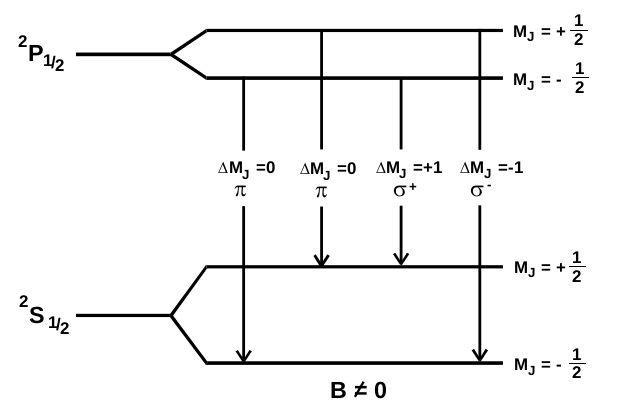
\includegraphics[width=0.9\columnwidth]{pictures/niveaus.png}
  \caption{Schematische Darstelllugn der Niveauaufspaltung eines Atom.\cite{Anleitung}}
  \label{fig:übergaenge_alkali}
\end{figure}
Dieser Prozess lässt sich gut anhand Abbildung \ref{fig:übergaenge_alkali}
erläutern.
Hierbei werden die Übergänge zwischen den beiden Zuständen $^2P_{\frac{1}{2}}$ und $^2S_{\frac{1}{2}}$ betrachtet.
Jedem Strahlenübergang, welcher jeweils die Auswahlregel $\Delta M_{\mathrm{J}} = 0, \pm 1$ erfüllt, ist eine Energie und ein Polarisationszustand zugeordnet.
Bei den beiden $\pi$-Übergängen wird jeweils linear polarisiertes Licht
emittiert bzw. absorbiert. Des Weiteren entspricht der $\sigma^+$-Übergang
rechtszirkular- und der $\sigma^-$-Übergang linkszirkular-polarisiertem Licht.
Wenn nun, wie beim Versuch, D$_1$-Licht (rechtszirkular-polarisiert)
eingestrahlt wird, werden die Elektronen nach der Absorption aus
dem Niveau $^2S_{\frac{1}{2}}, M_J = -\frac{1}{2}$ in das Niveau
$^2P_{\frac{1}{2}}, M_J = +\frac{1}{2}$ übergehen. Dabei ist eine
spontane Emission möglich, bei der das Elektron unter Emission eines
Photons in den vorherigen Zustand zurückkehrt. Allerdings liegt nach
der Planckschen Formel für die Frequenzabhängigkeit der
Übergangwahrscheinlichkeit bei einem spontanen Prozess von $\nu^3$ vor, sodass
spontane Prozesse erst für hohe Frequenzen zu berücksichtigen sind.
Es überwiegen also induzierte Prozesse. Damit ist es theoretisch möglich
das energetisch günstigere  $^2S_{\frac{1}{2}}, M_{\mathrm{J}} = -\frac{1}{2}$ Niveau
mit D$_1$-Licht leerzupumpen.

Bei dem Versuch wird die Transparenz, also die transmittierte Intensität
des D$_1$-Lichtes, verwendet, um die Übergänge zwischen den Zeemann-Niveaus
zu messen.
Ein typischer Verlauf der Transparenz gegen das anliegende Magnetfeld
ist in Abbildung \ref{fig:transparenz} dargestellt.
\begin{figure}
  \centering
  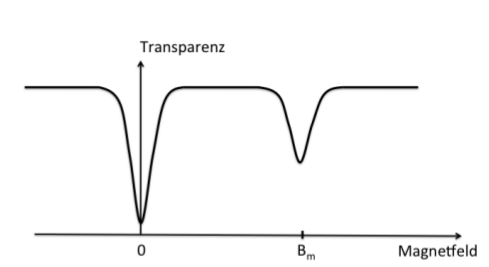
\includegraphics[width=0.9\columnwidth]{pictures/transparenz.png}
  \caption{Darstellung eines typischen Transparenzverlaufs der Dampfzelle in Abhängigkeit vom angelegten RF-Wechselfeld. \cite{Anleitung}}
  \label{fig:transparenz}
\end{figure}
Um den Wert $B=0$ fällt die Transparenz offensichtlich ab, weil dort
kein Zeemann-Effekt auftritt.
Zunächst wird mit dem D$_1$-Licht die Besetzungsinversion erzeugt, sodass
das energetisch günstigere Niveau nahezu leer ist. Damit können keine
durch das D$_1$-Licht iinduzierten Übergänge stattfinden, sodass die
Transparenz maximal wird. Nun ermöglicht das frequenzvariable
Wechselfeld (RF-Feld) eine induzierte Emission bei
\begin{equation}
	\label{eqn:g_f}
	B_{\mathrm{m}} = \frac{4\pi \mathrm{m}_0}{\mathrm{e}_0 g_J}\cdot \nu \mathrm{,}
\end{equation}
wobei $\mathrm{m}_0$ der Elektronenmasse \cite{m_0}, $\mathrm{e}_0$ der
Elementarladung \cite{e} und $\nu$ der angelegten Frequenz entspricht.
Bei dieser Resonanzfrequenz $\nu$ wird die Inversion rückgängig gemacht.
Und das energetisch günstigere Niveau ist wieder besetzt, was sich auch
bei der Transparenz bemerkbar macht, die einen weiteren negativen Peak
erfährt, der durch die wieder ermöglichten Absorptionen des D$_1$-Lichts durch das
$^2S_{\frac{1}{2}}, M_J = -\frac{1}{2}$ Niveau bedingt ist.
\subsection{Quadratischer Zeeman-Effekt}
Unter der Verwendung von Magnetfeldern mit großen Feldstärken müssen zur Beschreibung der Übergangsenergie $U_{\mathrm{HF}}$ weitere Terme höherer Ordnung berücksichtigt werden.
Dies ist notwendig, da bei großen Magnetfeldern der sogenannte Paschen-Back-Effekt eintritt, die Drehimpulse $\vec{J}$ sowie $\vec{I}$ einzeln an das Magnetfeld koppeln.
Unter der Berücksichtigung von Korrekturtermen quadratischer Ordnung ergibt sich für die Übergangsenergie $U_{\mathrm{HF}}$:
\begin{equation}
\label{eqn:quadrat_zeeman}
U_{\mathrm{HF}}=g_{\mathrm{F}}\mu_{\mathrm{B}}B+g_{\mathrm{F}}^2\mu_{\mathrm{B}}^2B^2\, \frac{\left(1-2\mathrm{M_F}\right)}{\Delta E_{\mathrm{Hy}}}	\mathrm{.}
\end{equation}
Es ist hierbei ist $\Delta E_{\mathrm{Hy}}$ die Energiedifferenz in der Hyperfeinstruktur sowie $M_{\mathrm{F}}$ die Gesamtdrehimpulsquantenzahl des betrachteten Atoms ist.
